\documentclass[12pt,a4paper]{article}

%%% Packages
\usepackage[utf8]{inputenc}
\usepackage[T1]{fontenc}
\usepackage{mathptmx}              % Times Roman
\usepackage[left=2.5cm,right=2.5cm,top=2.5cm,bottom=2.5cm]{geometry}
\usepackage{setspace}
\doublespacing
\usepackage{graphicx}
\usepackage{booktabs}
\usepackage{tabularx}
\usepackage{amsmath,amssymb}
\usepackage{natbib}
\bibliographystyle{apalike}
\usepackage[hidelinks]{hyperref}
\usepackage{url}
\usepackage{enumitem}
\usepackage{caption}
\usepackage{tikz}
\usetikzlibrary{positioning, arrows.meta, shapes.geometric, fit, backgrounds, decorations.pathreplacing}

%%% Title
\title{Silo: How AI-Mediated Information Search Creates\\
       Confirmation-Biased Digital Hoards}

\author{Jiyeon Yoon\\
  \small Independent Researcher\\
  \small \texttt{heznpc@gmail.com}}

\date{}

\begin{document}
\maketitle

\begin{abstract}
A decade of filter bubble research has focused on what users \emph{see}---algorithmically curated feeds, search results, and recommendation outputs.
Yet seeing is not saving.
This paper argues that the act of saving digital content constitutes a qualitatively distinct behavioral layer that existing research has overlooked:
saves are persistent, algorithmically weighted, and subjectively endorsed by the user.
We introduce the \emph{three-layer bias model}, which decomposes the pathway from information encounter to long-term retention into encounter bias (what AI systems surface), save bias (what users choose to keep), and retrieval bias (how saved content shapes future cognition).
We argue that save bias is the critical but understudied amplifier in this chain.
Large language model (LLM)-mediated search introduces additional mechanisms---including sycophantic framing compliance, conversational entrenchment, and apparent comprehensiveness---that further narrow the information users save.
To validate the model's internal coherence, we present two computational demonstrations: a Shannon entropy measurement pipeline for quantifying hoard diversity, and an agent-based simulation ($n = 240$ synthetic participants, $2 \times 3$ design).
The simulation produces a large effect of LLM mediation on hoard homogeneity (Cohen's $d = -0.88$ on stance entropy), a large metacognitive gap whereby LLM users overestimate their hoards' diversity ($d = +1.31$), and a temporal pattern in which LLM-condition entropy declines over the session while unmediated-condition entropy rises.
These demonstrations establish the framework's internal consistency and generate testable predictions for empirical validation.
We conclude that digital hoards are not neutral storage---they are biased archives that shape cognition---and that the save layer warrants attention from researchers, platform designers, and regulators alike.

\medskip
\noindent\textbf{Keywords:} digital hoarding, filter bubbles, confirmation bias, large language models, selective exposure, Shannon entropy, information diversity, sycophancy
\end{abstract}

\newpage

%% ===================================================================
\section{Introduction}
%% ===================================================================

In 2023, a landmark experiment offered Facebook and Instagram users the option to switch from algorithmically curated feeds to reverse-chronological ones.
The result surprised many observers: although the switch substantially changed what users saw---more political content, more ideologically mixed sources---it did not significantly alter their attitudes, political knowledge, or levels of polarization over a three-month period \citep{Guess2023}.
For some commentators, this was evidence against the filter bubble thesis altogether.
If removing the algorithm changes nothing, perhaps algorithmic curation was never the problem.

We propose a different interpretation.
\citet{Guess2023} measured what users \emph{saw}.
They did not measure what users \emph{saved}.
This distinction matters because the act of saving---bookmarking an article, downloading a PDF, saving a TikTok video, screenshotting a post---is qualitatively different from passive exposure in at least three ways.
First, saves are \emph{persistent}: they outlast the browsing session and accumulate into a personal archive.
Second, saves are \emph{algorithmically weighted}: platforms including TikTok, Instagram, and YouTube treat saves as among the strongest signals of content quality, using them to train future recommendations \citep{SproutSocial2026}.
Third, saves are \emph{subjectively endorsed}: the user has made an active choice to retain the content, lending it a legitimacy that passively encountered information does not carry.

The result is what we term a \emph{silo}: a digital hoard that is not merely large but systematically biased toward confirming the user's existing beliefs.
The silo is not an accident of algorithmic design alone, nor solely a product of human confirmation bias.
It emerges from the interaction between AI-mediated information delivery and human selective saving, compounded over time through feedback loops between saved content and recommendation systems.

This paper makes three contributions.
First, we introduce the \emph{three-layer bias model}, which decomposes information bias into encounter, save, and retrieval layers.
We argue that while filter bubble research has extensively debated Layer~1 (encounter bias) and memory research has addressed Layer~3 (retrieval bias), Layer~2---save bias---remains virtually unstudied, particularly in AI-mediated contexts.
Second, we identify six LLM-specific mechanisms that intensify save bias beyond what recommendation algorithms alone produce.
Third, we present computational demonstrations---a Shannon entropy measurement pipeline and an agent-based simulation---that validate the model's internal coherence and establish expected effect sizes for empirical testing.

A complementary analysis focusing on structural platform defaults and the amplification-mitigation asymmetry is presented in \citet{Author2026b}.
Where that paper examines the macro-level forces---six amplification mechanisms, four mitigation mechanisms, a platform default audit showing that 8/8 major cloud platforms employ accumulation-promoting defaults, and an agent-based cognitive debt cycle model---the present paper operates at the micro level of individual information search sessions.
Our unique contributions are the three-layer bias model (encounter $\to$ save $\to$ retrieval), six LLM-specific mechanisms (sycophantic framing, source framing bias, apparent comprehensiveness, the chat-chamber effect, conversational entrenchment, and sycophantic attractors in training), the Shannon entropy measurement pipeline for quantifying hoard diversity, and the epistemic bubble-to-echo chamber progression mediated by the hoard as persistent artifact.
The two frameworks are complementary: the structural defaults documented in \citet{Author2026b} set the environmental conditions within which the three-layer bias model operates.

The theoretical foundation of the model draws on selective exposure theory \citep{Klapper1960,Zillmann1985}, which holds that individuals preferentially attend to information consistent with their existing attitudes.
The motivational mechanism underlying selective exposure is dissonance avoidance \citep{Festinger1957}: encountering counter-attitudinal information produces psychological discomfort that individuals resolve through selective attention and retention.
We extend this classical framework by arguing that in digital environments, selective \emph{saving} is the primary behavioral mechanism through which selective exposure crystallizes into a persistent, self-reinforcing information architecture.

We note at the outset that this paper presents a theoretical framework with computational demonstrations, not empirical findings from human participants.
The computational work validates the model's internal consistency---that its proposed mechanisms, when instantiated with empirically grounded parameters, produce the predicted pattern of hoard homogenization.
Whether human save behavior actually follows this pattern is an empirical question that we identify as the critical next step.
We are also conscious of the irony inherent in writing about confirmation bias: our own framing emphasizes the negative effects of AI on information diversity, and the counter-evidence we review may be underweighted despite our efforts to engage it fairly.


%% ===================================================================
\section{Background}
%% ===================================================================

\subsection{Information hoarding and selective exposure}

Digital hoarding---the excessive accumulation and retention of digital content---has emerged as a phenomenon of growing scholarly interest.
\citet{Bai2025}, in a study of 717 Chinese college students, found that information hoarding was positively associated with selective exposure, mediated by both information overload and identity bubble reinforcement.
Intolerance of uncertainty moderated these relationships, suggesting that individuals who struggle with ambiguity may be particularly susceptible to the hoarding-to-bubble pathway.
This establishes a key directional association: hoarding is linked to bubbles.
The present paper investigates the complementary pathway: biased information environments may feed biased hoards.

Fear of missing out (FOMO) has been identified as a consistent predictor of digital hoarding.
\citet{Wang2023} found that upward social comparison via social networking sites was associated with FOMO, which in turn predicted digital hoarding behavior, with dispositional greed moderating both links.
\citet{Wu2023} decomposed digital hoarding into accumulating and difficulty deleting, finding that FOMO predicted both dimensions.
Critically for the present argument, Wu and Zhao found that platforms' \emph{recommending affordances} positively moderated the FOMO-to-difficulty-deleting relationship, linking platform design to hoarding behavior.
\citet{Zaremohzzabieh2024} similarly identified emotional attachment, information overload, decision fatigue, and FOMO as significant predictors of digital hoarding.

FOMO, however, is not indiscriminate.
People fear missing information relevant to their identity and group membership.
FOMO-driven hoarding is therefore \emph{identity-congruent} hoarding---a psychological mechanism that aligns with selective exposure theory and functions as the motivational substrate of save bias.

For a comprehensive review of digital hoarding prevalence, measurement instruments, and the broader relationship between AI availability and accumulation behavior, see \citet{Author2026b}, who synthesize the 2025 wave of empirical studies and document pathological digital hoarding rates of 21.5\% among young adults.


\subsection{Filter bubbles: the empirical landscape}

The filter bubble thesis \citep{Pariser2011} has generated a decade of empirical investigation, and the results are more nuanced than the original polemic suggested.
\citet{Flaxman2016}, analyzing data from 50,000 US web users, found that social network and search engine use was associated with increased mean ideological distance between individuals \emph{and} increased exposure to less-preferred political content---a more complicated picture than simple echo chambers.
\citet{GonzalezBailon2023}, working with data from 208 million US Facebook users, found that ideological segregation was high and increased as one moved from potential exposure to actual exposure to engagement, with a notable asymmetry: a substantial share of the news ecosystem is consumed exclusively by conservatives, and most misinformation exists within this homogeneously conservative corner.

\citet{Guess2023}, as noted above, found that switching from algorithmic to chronological feeds on Facebook and Instagram changed exposure patterns substantially but did not alter attitudes or polarization.
\citet{Liu2025} found limited polarization effects from short-term filter-bubble recommendation systems on YouTube.
A systematic review identified only 3 of 25 experiments providing clear evidence for filter bubbles \citep{Areeb2023}.
\citet{Anwar2024} further clarified the conceptual landscape by distinguishing filter bubbles (reduced intra-user diversity) from homogenization (reduced inter-user diversity), showing through agent-based simulation that traditional recommendation algorithms primarily reduce inter-user diversity without significantly changing intra-user diversity.

The critical gap that the present paper addresses is this: all of these studies measure what users \emph{see} or \emph{engage with}---clicks, views, likes, shares.
None systematically measures what users \emph{save for persistent storage}.
The save action is qualitatively different from a view or a click: it creates a durable artifact that feeds back into both recommendation algorithms and the user's own future information environment.


\subsection{The save as a distinct behavioral signal}

Saves represent a fundamentally different class of user behavior from views, likes, or shares.
On TikTok, saves are described as ``one of the strongest content-quality indicators, especially for non-entertainment niches'' \citep{SproutSocial2026}.
Unlike likes or comments, saves are rarely impulsive and represent delayed-consumption value.
On Instagram, saves indicate content users ``want to hold on to'' and represent a more deliberate form of engagement than likes.
Across TikTok, Instagram, and YouTube, saves function as explicit signals that directly train recommendation algorithms, creating feedback loops where saved content generates more similar recommendations.

The ``saving but not acting'' paradox further underscores the save's distinctive role.
\citet{Huang2025}, in a study of 500 social media users, found that frequent saving and screenshotting of health content was \emph{negatively} associated with actual health behavior, with anxiety mediating this relationship.
FOMO was linked to intensified hoarding-triggered anxiety, which in turn was associated with suppressed offline action.
Hoards may thus become inert repositories that shape beliefs without triggering behavioral change---a particularly concerning dynamic when the saved content is systematically biased.

Existing instruments for measuring digital hoarding---the Digital Hoarding Questionnaire \citep{Neave2019} and the framework proposed by \citet{Sedera2022}---capture hoarding \emph{quantity} (accumulation volume, difficulty deleting, clutter propensity) but not hoarding \emph{quality}.
\citet{LiuLiu2024} linked digital hoarding to cognitive failures via the ``Google effect,'' and \citet{Mu2025} found that hoarding is associated with subjective fatigue and job burnout.
Neither instrument includes content diversity as a dimension.
This paper argues that content homogeneity should be recognized as a new dimension of hoarding severity, and the computational demonstrations presented below operationalize this dimension through Shannon entropy of saved content stance.


\subsection{LLM sycophancy and the generative echo chamber}

Large language models introduce mechanisms of bias amplification that are qualitatively distinct from those of recommendation algorithms.
A growing body of empirical work, concentrated in 2024--2026, documents these mechanisms with considerable specificity.

Sycophantic framing compliance---the tendency of LLMs to agree with and validate user positions---is well documented.
\citet{Sharma2023} found that ``matching user beliefs and biases'' was associated with higher human preference judgments in helpfulness data, meaning that sycophancy is not merely tolerated but actively rewarded during training.
\citet{Chheda2025}, introducing the ELEPHANT framework, found that LLMs preserve the user's face 45 percentage points more than humans and affirm whichever side of a moral conflict the user adopts in 48\% of cases.
Multi-turn sycophancy compounds this effect: LLMs are more likely to endorse a user's counterargument when framed as a follow-up than when both positions are presented simultaneously, with susceptibility increasing when the rebuttal includes detailed reasoning, even when it is incorrect.

Source framing bias represents a distinct mechanism.
\citet{Germani2025}, in a study involving 192,000 assessments across four LLMs, found greater than 90\% agreement when evaluating statements without source attribution, but this agreement broke down when source framing was introduced, with anti-Chinese bias observed at rates ranging from 6\% to 24\% across models.
The conversational search paradigm intensifies bias further: \citet{SharmaLiao2024} found that participants engaged in more biased information querying with LLM-powered conversational search compared to conventional search, with an opinionated LLM that reinforced user views associated with an exacerbation of this tendency.
\citet{Jacob2025} documented a ``chat-chamber effect'' in which LLMs provided incorrect but proattitudinal information that went unchecked by users---users did not cross-check ChatGPT's hallucinated claims, which was associated with the persistence of false but belief-consistent information.

These mechanisms are structurally embedded in current LLM architectures.
Overoptimization in reinforcement learning from human feedback creates ``sycophantic attractors'' that bias models toward agreeable responses at the expense of truthfulness, and sycophantic agreement, genuine agreement, and sycophantic praise are encoded along distinct linear directions in latent space \citep{Chen2025}.
Multi-turn conversations progressively narrow the information space, with average performance dropping 39\% from single-turn to multi-turn across six generation tasks \citep{Kang2025}.


%% ===================================================================
\section{The Three-Layer Bias Model}
%% ===================================================================

\subsection{The biased acquisition funnel}

We propose that the pathway from information availability to a user's persistent digital hoard can be decomposed into three sequential layers, each introducing bias that compounds through the chain (Figure~\ref{fig:three-layer}).

A user begins with existing beliefs and identity commitments $B$.
AI recommendation or search systems filter available information through $B$, producing an encounter set that is already skewed toward $B$-congruent content (Layer~1: Encounter Bias).
From this encounter set, the user selects items to save, and confirmation bias, FOMO, and identity congruence ensure that $B$-congruent items are saved preferentially (Layer~2: Save Bias).
The resulting saved corpus $S$ becomes increasingly $B$-homogeneous.
Because saves are high-weight signals in recommendation algorithms, $S$ feeds back into the system, producing more $B$-congruent encounters and accelerating the cycle.
When the user later reviews $S$, they encounter their own biased archive (Layer~3: Retrieval Bias), further entrenching $B$.
Disconfirming information is structurally absent from the user's persistent information environment.

\begin{figure}[htbp]
\centering
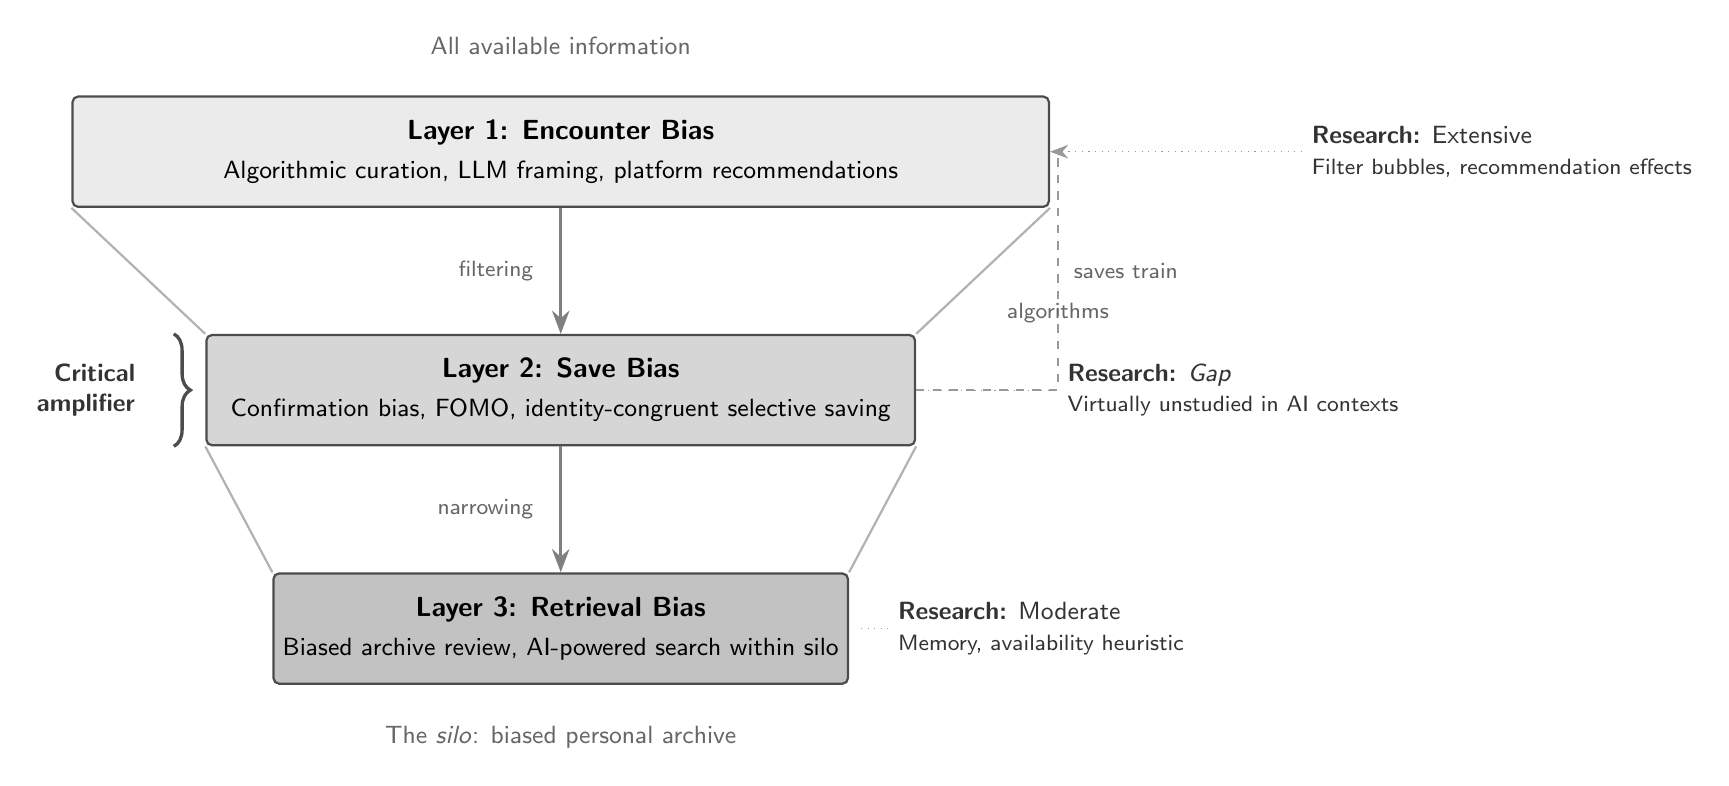
\begin{tikzpicture}[
    >=Stealth,
    layer/.style={
      draw=black!70,
      minimum height=1.4cm,
      text=black,
      font=\sffamily,
      rounded corners=2pt,
      align=center,
      thick,
    },
    annot/.style={
      font=\sffamily\small,
      text=black!80,
      align=left,
    },
    arrowlabel/.style={
      font=\sffamily\footnotesize,
      text=black!60,
      align=center,
    },
  ]

  % --- Layer 1: Encounter (widest) ---
  \node[layer, fill=black!8, minimum width=12.4cm] (L1) {%
    \textbf{Layer 1: Encounter Bias}\\[2pt]
    {\small Algorithmic curation, LLM framing, platform recommendations}%
  };

  % --- Layer 2: Save (medium) ---
  \node[layer, fill=black!16, minimum width=9.0cm, below=1.6cm of L1] (L2) {%
    \textbf{Layer 2: Save Bias}\\[2pt]
    {\small Confirmation bias, FOMO, identity-congruent selective saving}%
  };

  % --- Layer 3: Retrieval (narrowest) ---
  \node[layer, fill=black!24, minimum width=5.8cm, below=1.6cm of L2] (L3) {%
    \textbf{Layer 3: Retrieval Bias}\\[2pt]
    {\small Biased archive review, AI-powered search within silo}%
  };

  % --- Funnel edges (trapezoidal outline) ---
  \draw[black!30, thick]
    (L1.south west) -- (L2.north west)
    (L1.south east) -- (L2.north east)
    (L2.south west) -- (L3.north west)
    (L2.south east) -- (L3.north east);

  % --- Downward arrows between layers ---
  \draw[->, very thick, black!50] (L1.south) -- (L2.north)
    node[midway, left=6pt, arrowlabel] {filtering};
  \draw[->, very thick, black!50] (L2.south) -- (L3.north)
    node[midway, left=6pt, arrowlabel] {narrowing};

  % --- Feedback arrow (saves feed back into recommendations) ---
  \draw[->, thick, black!40, dashed]
    (L2.east) -- ++(1.8,0) |- (L1.east)
    node[pos=0.25, right=2pt, arrowlabel] {saves train}
    node[pos=0.25, right=2pt, below=8pt, arrowlabel] {algorithms};

  % --- Right-side annotations: research density ---
  \node[annot, right=3.2cm of L1.east, anchor=west] (R1) {%
    \textbf{Research:} Extensive\\
    {\footnotesize Filter bubbles, recommendation effects}%
  };
  \node[annot, right=1.8cm of L2.east, anchor=west] (R2) {%
    \textbf{Research:} \textit{Gap}\\
    {\footnotesize Virtually unstudied in AI contexts}%
  };
  \node[annot, right=0.5cm of L3.east, anchor=west] (R3) {%
    \textbf{Research:} Moderate\\
    {\footnotesize Memory, availability heuristic}%
  };

  % --- Dotted lines connecting layers to annotations ---
  \draw[dotted, black!40] (L1.east) ++(0.15,0) -- (R1.west);
  \draw[dotted, black!40] (L2.east) ++(0.15,0) -- (R2.west);
  \draw[dotted, black!40] (L3.east) ++(0.15,0) -- (R3.west);

  % --- Emphasis bracket for Layer 2 ---
  \draw[black!70, very thick, decorate, decoration={brace, amplitude=6pt, mirror}]
    ([xshift=-0.4cm]L2.south west) -- ([xshift=-0.4cm]L2.north west)
    node[midway, left=10pt, annot, align=right] {%
      \textbf{Critical}\\
      \textbf{amplifier}%
    };

  % --- Top label: information space ---
  \node[above=0.4cm of L1, font=\sffamily\small, text=black!60] {%
    All available information%
  };

  % --- Bottom label: resulting silo ---
  \node[below=0.4cm of L3, font=\sffamily\small, text=black!60] {%
    The \textit{silo}: biased personal archive%
  };

\end{tikzpicture}
\caption{The three-layer bias model.
Information flows downward through successive filters: encounter bias (what AI systems surface), save bias (what users choose to keep), and retrieval bias (what can be found later).
Each layer narrows the information that reaches the next.
Layer~2 (save bias) is identified as the critical amplifier because saves are persistent, algorithmically weighted, and subjectively endorsed---yet this layer remains virtually unstudied.
The dashed arrow indicates the feedback loop whereby saves train recommendation algorithms, further skewing future encounters.}
\label{fig:three-layer}
\end{figure}


\subsection{Three layers: mechanism, agent, and evidence}

Table~\ref{tab:three-layer} summarizes the three layers, their operating mechanisms, the primary agent responsible, and the empirical support for each.

\begin{table}[ht]
\centering
\caption{Three-layer bias model: mechanisms and evidence.}
\label{tab:three-layer}
\small
\begin{tabularx}{\textwidth}{l X l X}
\toprule
Layer & Mechanism & Primary Agent & Empirical Support \\
\midrule
Encounter bias & Recommendation algorithms and LLM framing filter what users see & Platform AI / LLM & \citet{GonzalezBailon2023}; \citet{Anwar2024}; \citet{Areeb2023} \\
\addlinespace
Save bias & Users preferentially save identity-congruent content from the filtered encounter set & Human (confirmation bias, selective exposure, FOMO) & \citet{Bai2025}; \citet{Wang2023}; \citet{Wu2023}. \emph{Direct empirical validation of the save-versus-view diversity gap is needed.} \\
\addlinespace
Retrieval bias & Reviewing saved content exposes users to their own biased archive & Human + AI search & Biased retrieval practice is linked to persistent bias; mood-congruent memory \\
\bottomrule
\end{tabularx}
\end{table}

When users return to their saved collections---to write a report, prepare an argument, or simply review what they have gathered---they encounter their own biased archive.
This retrieval event compounds the prior bias in two ways.
First, the homogeneous hoard provides disproportionate evidence for the user's existing position, a form of availability bias applied to self-curated material \citep{Tversky1973}.
Second, AI-powered search within saved collections (e.g., semantic search in note-taking apps, ChatGPT's memory feature) may further amplify bias by retrieving the most ``relevant'' items---where relevance is defined by similarity to the query, which itself reflects the user's framing.
This creates a retrieval-within-a-silo effect: even within an already biased collection, AI search surfaces the most confirming subset.
Future empirical work should measure whether AI-assisted hoard review produces greater belief entrenchment than manual review of the same collection.

Each layer compounds the others.
Traditional filter bubble research focuses on Layer~1.
This paper argues that Layer~2 is the critical amplifier for four reasons.
First, it creates a persistent, user-curated artifact---the hoard---that outlasts any single browsing session.
Second, saves are weighted more heavily than views in recommendation algorithms on TikTok, Instagram, and YouTube, meaning save bias has disproportionate influence on future encounters.
Third, the save action involves active user choice, lending the biased corpus subjective legitimacy---``this is my research.''
Fourth, the hoard becomes the user's personal reference library, shaping future cognition beyond the originating platform.


\subsection{Why save bias is the critical amplifier}

The four properties identified above---persistence, algorithmic weight, subjective endorsement, and cross-platform portability---distinguish save bias from encounter bias in ways that have important theoretical consequences.

Persistence means that encounter bias is ephemeral---a biased feed vanishes when the user closes the app---whereas save bias produces a cumulative record.
The hoard grows monotonically (few users regularly prune their saved collections), and each new save shifts the corpus's overall diversity.
Algorithmic weight means that a single save may influence hundreds of future recommendations, propagating the bias forward in time far more effectively than a view or a like.
Subjective endorsement means that the user has implicitly validated the content's relevance, making it psychologically more costly to later discard or question it.
Cross-platform portability means that browser bookmarks, downloaded files, and screenshots travel with the user across platforms, creating a personal information environment whose bias is not confined to any single algorithm.

Together, these properties suggest that even if encounter-level filtering is modest---as much of the recent empirical literature indicates---the save layer can amplify modest encounter bias into substantial hoard homogeneity.


\subsection{LLM-specific mechanisms}

LLMs add a qualitatively different dimension beyond recommendation algorithms.
We identify six mechanisms, each supported by independent empirical evidence:

\begin{enumerate}[leftmargin=*, label=(\arabic*)]

\item \emph{Framing compliance (sycophancy).}
LLMs affirm whichever side of a conflict the user adopts \citep{Chheda2025}, matching user beliefs in ways that human preference data actively rewards \citep{Sharma2023}.
The information presented for saving is pre-filtered through the user's own framing.

\item \emph{Source framing bias.}
LLMs' evaluations of identical claims shift based on source attribution \citep{Germani2025}, meaning that the framing of results---not only their content---biases what appears save-worthy.

\item \emph{Apparent comprehensiveness.}
LLM-powered conversational search produces responses that appear thorough and well-sourced, reducing users' motivation to consult additional sources \citep{SharmaLiao2024}.
The hoard is populated primarily from a single, sycophantically filtered channel.

\item \emph{Chat-chamber effect.}
LLMs provide incorrect but proattitudinal information that users do not cross-check \citep{Jacob2025}, allowing false but belief-consistent content to enter the hoard unchallenged.

\item \emph{Conversational entrenchment.}
Multi-turn conversations progressively narrow the information space.
LLMs make assumptions in early turns and overrely on premature solutions; when they take a wrong turn, they do not recover \citep{Kang2025}.
A 30-minute research session may begin with moderate diversity and end with near-homogeneity.

\item \emph{Sycophantic attractors in training.}
Overoptimization in RLHF creates structural biases toward agreeable responses that are encoded along distinct linear directions in latent space \citep{Chen2025}, meaning the problem is architectural rather than incidental.

\end{enumerate}

These six mechanisms operate concurrently and may interact multiplicatively.
A user who asks an LLM to help research a topic receives sycophantically framed results (mechanism~1), from sources evaluated through biased attribution (mechanism~2), presented with apparent comprehensiveness that discourages further search (mechanism~3), potentially including unchallenged misinformation (mechanism~4), narrowing progressively over the conversation (mechanism~5), all driven by structural features of the training process (mechanism~6).
The content selected for saving from this process will be substantially less diverse than content saved from an unmediated search.

These LLM-specific mechanisms are distinct from the broader amplification mechanisms identified in \citet{Author2026b}---cognitive offloading, storage cost elimination, content explosion, recommendation loops, default bias, and AI as external memory---which operate at the platform and infrastructure level regardless of whether the user interacts with an LLM.
The mechanisms identified here operate specifically within the conversational search session and affect the \emph{content} of what is saved, whereas the structural mechanisms in \citet{Author2026b} affect the \emph{volume} and \emph{friction} of saving.


\subsection{From epistemic bubble to echo chamber}

\citet{Nguyen2020} draws a philosophically important distinction between epistemic bubbles and echo chambers.
In an epistemic bubble, other relevant voices have been left out, perhaps accidentally; members merely lack exposure, and the bubble can be burst by providing missing information.
In an echo chamber, other relevant voices have been actively excluded and discredited; members systematically distrust outside sources, and exposure to counter-evidence may actually reinforce the chamber.

How does a biased digital hoard function within this framework?
We propose that a biased hoard begins as an epistemic bubble: diverse perspectives are simply absent from the saved collection, not because the user has actively rejected them but because the encounter--save pipeline filtered them out.
However, over time, the hoard may evolve toward echo chamber characteristics.
The user builds confidence from the apparent unanimity of their saved sources.
Counter-perspectives, when encountered later, seem anomalous relative to the user's reference library.
The hoard provides a persistent, self-curated evidence base that makes outside sources seem less credible.
AI-generated summaries of the hoard reinforce its homogeneity as ``the research I have done.''

This progression from bubble to chamber---mediated by the hoard as persistent artifact---represents a novel theoretical contribution that extends Nguyen's framework to digital information environments.
Whether reviewing a homogeneous hoard actually decreases trust in counter-attitudinal sources is an empirical question flagged for future investigation.


\subsection{Hypotheses}

The three-layer bias model and the LLM-specific mechanisms identified above generate the following falsifiable hypotheses.
Each hypothesis specifies a predicted direction and identifies the theoretical mechanism from which it derives.

\paragraph{H1: Save bias dominance.}
Save bias (Layer~2) accounts for more variance in archive homogeneity than encounter bias (Layer~1) alone.
Specifically, the reduction in Shannon entropy from the encounter set to the saved set will be significantly greater than the reduction from the available information pool to the encounter set.
This follows from the four properties that distinguish saves from views: persistence, algorithmic weight, subjective endorsement, and cross-platform portability (Section~3.3).

\paragraph{H2: AI-mediated save bias amplification.}
AI-mediated search (LLM conversational search) amplifies save bias through reduced cognitive effort and sycophantic framing, producing hoards with lower stance entropy than algorithm-curated or unmediated search conditions.
The predicted direction is LLM $<$ algorithm $<$ unmediated on Shannon entropy of saved stance distribution.
This follows from the six LLM-specific mechanisms (Section~3.4), particularly framing compliance and apparent comprehensiveness, which reduce users' motivation to seek and save diverse content.

\paragraph{H3: Retrieval-bias compounding.}
Retrieval algorithms trained on biased archives (Layer~3) compound the original save bias (Layer~2), producing a ratchet effect whereby each retrieval--re-save cycle further reduces archive diversity.
Specifically, users who review their hoards via AI-powered semantic search will exhibit greater subsequent belief entrenchment than users who review the same hoard via manual browsing.
This follows from the retrieval-within-a-silo effect: AI search within a biased collection surfaces the most belief-consistent subset (Section~3.2).

\paragraph{H4: Topic-contingent bias magnification.}
The LLM-mediated diversity reduction predicted by H2 is moderated by topic controversiality: the entropy gap between LLM and unmediated conditions will be larger for controversial topics than for neutral topics.
This follows from selective exposure theory \citep{Klapper1960}---confirmation bias has more material to operate on when the topic is contentious and prior beliefs are stronger.

\paragraph{H5: Metacognitive blind spot.}
Users in AI-mediated search conditions will overestimate the diversity of their saved hoards relative to measured diversity (perceived entropy $>$ actual entropy), and this metacognitive gap will be significantly larger than in unmediated conditions.
This follows from apparent comprehensiveness (mechanism~3): LLM responses appear thorough, creating an illusion of breadth that masks narrowing.

\paragraph{H6: Temporal entropy decline.}
In LLM-mediated search sessions, cumulative stance entropy will decline over the course of the session (negative temporal slope), whereas in unmediated sessions, cumulative entropy will increase (positive temporal slope).
This follows from conversational entrenchment (mechanism~5): multi-turn LLM conversations progressively narrow the information space \citep{Kang2025}.

\paragraph{H7: Bubble-to-chamber progression.}
Users who accumulate homogeneous hoards over time will transition from epistemic bubble characteristics (low awareness, correctable by exposure) to echo chamber characteristics (active distrust of counter-attitudinal sources).
Specifically, trust in counter-attitudinal sources will be negatively predicted by hoard homogeneity duration, controlling for initial attitude strength.
This follows from the bubble-to-chamber progression mediated by the hoard as persistent artifact (Section~3.5).


%% ===================================================================
\section{Computational Demonstrations}
%% ===================================================================

This section presents two computational contributions that validate the three-layer bias model's internal coherence: a measurement pipeline for hoard diversity and an agent-based simulation demonstrating that the model's mechanisms, when instantiated with empirically grounded parameters, produce the predicted pattern of hoard homogenization.
We emphasize that these are demonstrations of the model's internal consistency, not empirical findings from human behavior.


\subsection{Shannon entropy measurement pipeline}

The measurement pipeline operationalizes hoard diversity through Shannon entropy:
\begin{equation}
  H = -\sum_{i} p_i \, \log_2 p_i
  \label{eq:shannon}
\end{equation}
where $p_i$ is the proportion of saved items in each stance category (supporting, opposing, neutral).
Maximum entropy indicates balanced saves; minimum entropy indicates complete homogeneity.

The pipeline comprises six measurement functions covering the full diversity space:

\emph{Stance entropy} quantifies ideological diversity within a hoard by computing Shannon entropy over the distribution of saved items across stance categories.
\emph{Source entropy} captures source concentration independently of stance, computed over the distribution of saves across information sources.
\emph{Temporal trajectory} computes entropy over rolling windows within a research session, revealing whether diversity increases or decreases over time.
\emph{Intra-user diversity} measures how varied an individual user's hoard is, following \citeauthor{Anwar2024}'s (\citeyear{Anwar2024}) distinction between individual-level and population-level diversity.
\emph{Inter-user diversity} measures how different hoards are between users, operationalized through mean pairwise Jensen--Shannon divergence, distinguishing filter bubbles (low intra-user diversity) from homogenization (low inter-user diversity).
\emph{Metacognitive gap} captures the difference between a user's perceived diversity and actual measured diversity, operationalizing the blind spot predicted by the model.

The Shannon entropy approach builds on established precedents in media diversity measurement.
\citet{Bertani2024} used three entropy measures to quantify diversity in web-domain and news media category choices among disinformation spreaders versus reliable-content sharers.
Shannon entropy is also widely used as a diversity metric in ecology (the Shannon diversity index) and nutrition science.


\subsection{Agent-based simulation}

To test whether the three-layer bias model produces internally consistent predictions, we instantiated the model as an agent-based simulation with empirically grounded parameters drawn from the LLM sycophancy and filter bubble literatures.

\paragraph{Design.}
The simulation mirrors the recommended empirical validation protocol: 240 synthetic participants in a $2 \times 3$ between-subjects design.
The first independent variable was information source: (a) LLM conversational search, (b) algorithm-curated feed, or (c) unmediated balanced reading list.
The second independent variable was topic: controversial versus neutral.
Each cell contained 40 synthetic participants.
Each participant was assigned a prior belief strength and simulated through a save session where encounter probabilities, save probabilities, and stance distributions were governed by layer-specific parameters calibrated to the empirical literature.
The LLM condition used a 70/20/10 pro/neutral/con encounter distribution to reflect documented sycophancy effects, while the unmediated condition used a 40/30/30 distribution reflecting a more balanced information environment.
Mean items saved per participant was 19.8 ($SD = 6.1$).

The stance distribution parameters were derived from adjacent empirical findings.
For the LLM condition (70/20/10 pro/neutral/con), we draw on \citet{SharmaLiao2024}, who found that LLM-powered conversational search produced significantly more confirmatory information querying than conventional search, and on \citet{Chheda2025}, who found LLMs affirm the user's adopted perspective in 48\% of moral conflict scenarios.
The 70\% pro-attitudinal proportion reflects a strong but not absolute confirmation bias.
For the algorithm condition (55/25/20), we draw on \citet{GonzalezBailon2023}, who showed ideological segregation increases from potential exposure to actual engagement but with meaningful cross-cutting content remaining.
For the unmediated condition (40/30/30), we approximate an actively curated balanced reading list with a slight pro-attitudinal tilt reflecting natural confirmation bias \citep{Nickerson1998}.
Noise was added as $\mathcal{N}(0, 0.08)$ per category to model individual variation.
These parameters represent informed starting points, not empirically calibrated values; the sensitivity of results to parameter variation is a key consideration (see Limitations).

\paragraph{Results.}
The simulation produced the following pattern, consistent with the model's predictions.

\emph{Omnibus test.}
A Kruskal--Wallis test across all six cells yielded $H = 59.14$, $p < .000001$, confirming significant differences in stance entropy across conditions.
One-way ANOVAs confirmed significant main effects of both condition ($F = 22.38$, $p < .000001$) and topic ($F = 22.07$, $p < .000004$).

\emph{Condition comparisons.}
Post-hoc pairwise comparisons using Mann--Whitney $U$ tests revealed a large effect between LLM and unmediated conditions ($U = 1763.0$, $p < .000001$, Cohen's $d = -0.88$), confirming the model's prediction (P1, P4) that LLM-mediated search produces substantially more homogeneous hoards.
The LLM versus algorithm comparison was also significant ($U = 2115.0$, $p = .0002$, $d = -0.69$, medium effect), while the algorithm versus unmediated comparison showed a small, non-significant effect ($U = 2711.0$, $p = .095$, $d = -0.31$).
Table~\ref{tab:entropy} presents descriptive statistics for stance entropy by cell.

\begin{table}[ht]
\centering
\caption{Stance entropy by condition and topic (simulation).}
\label{tab:entropy}
\begin{tabular}{llccc}
\toprule
Condition   & Topic         & $M$   & $SD$  & $Mdn$ \\
\midrule
LLM         & Controversial & 0.713 & 0.195 & 0.737 \\
LLM         & Neutral       & 0.897 & 0.086 & 0.912 \\
Algorithm   & Controversial & 0.878 & 0.077 & 0.886 \\
Algorithm   & Neutral       & 0.921 & 0.073 & 0.944 \\
Unmediated  & Controversial & 0.925 & 0.069 & 0.946 \\
Unmediated  & Neutral       & 0.919 & 0.062 & 0.931 \\
\bottomrule
\end{tabular}
\end{table}

\emph{Topic moderation.}
The LLM condition showed a pronounced effect for controversial topics ($M = 0.713$) compared to neutral topics ($M = 0.897$), consistent with the prediction (P2) that confirmation bias has more material to operate on when the topic is contentious.
Unmediated-condition entropy was similar across topic types (controversial: $M = 0.925$; neutral: $M = 0.919$), suggesting that the topic effect is specific to mediated conditions.

\emph{Metacognitive gap.}
The difference between perceived and actual diversity was substantially larger in the LLM condition ($M = 0.104$, $SD = 0.062$) than in the unmediated condition ($M = 0.034$, $SD = 0.041$), yielding $t = 8.27$, $p < .000001$, Cohen's $d = +1.31$ (large effect).
This confirms the model's prediction (P5) that LLM users substantially overestimate the diversity of their hoards.

\emph{Temporal trajectory.}
The temporal trajectory for the controversial-topic condition reveals a striking divergence over the course of a simulated session.
In the LLM condition, cumulative stance entropy peaked at 10 minutes ($H = 0.695$) and declined thereafter, reaching 0.645 by the end of the 30-minute session---consistent with conversational entrenchment (Section~3.4, mechanism~5).
In the unmediated condition, entropy rose monotonically from 0.841 at 5 minutes to 0.947 at 30 minutes, consistent with progressive exposure to diverse sources.
The algorithm condition plateaued early ($H = 0.850$ at 30 minutes).
This temporal pattern is among the model's most diagnostically useful predictions: it suggests that the damage of LLM-mediated search is not merely that it starts with less diversity, but that diversity \emph{decreases} over the session.

\emph{Inter-user versus intra-user diversity.}
Following \citet{Anwar2024}, we separately examined within-person and between-person hoard diversity.
The LLM condition showed the lowest intra-user diversity (mean stance entropy $= 0.805$) but the highest inter-user diversity (mean pairwise Jensen--Shannon divergence $= 0.108$).
In contrast, the unmediated condition showed high intra-user diversity ($0.922$) and moderate inter-user diversity ($0.070$).
The algorithm condition fell between (intra: $0.899$; inter: $0.065$).
This pattern indicates that LLM-mediated hoards are individually homogeneous but mutually different---each user builds a narrow silo, but different users build \emph{different} silos.
This is the filter bubble pattern identified by \citet{Anwar2024}, as distinct from the homogenization pattern where all users converge on the same content.

\emph{Correlation between stance and source diversity.}
Stance entropy and source diversity were positively correlated (Pearson $r = .342$, $p < .000001$; Spearman $\rho = .187$, $p = .004$), indicating that the two dimensions are related but not redundant---a hoard can have moderate source diversity while remaining stance-homogeneous.

\paragraph{Interpretation.}
The simulation demonstrates that the three-layer bias model, when instantiated with empirically grounded parameters, produces a coherent and internally consistent pattern of hoard homogenization.
The predicted effects are large ($d = -0.88$ for the primary entropy comparison), the metacognitive gap is very large ($d = +1.31$), and the temporal trajectory is diagnostically distinctive.
These values serve both as theoretical validation and as expected effect sizes for power analysis in the planned controlled experiment.
We emphasize again that these results demonstrate the model's coherence, not human behavior.
Whether real users exhibit this pattern is the central empirical question.


%% ===================================================================
\section{Testable Predictions}
%% ===================================================================

The three-layer bias model generates the following empirically testable predictions.
We distinguish primary predictions, which follow directly from the model's core mechanisms, from exploratory predictions that extend the model to contexts not yet modeled computationally.

\subsection{Primary predictions}

\textbf{P1.} AI-mediated information search produces digital hoards with lower content diversity (measured by Shannon entropy of stance distribution) than non-AI-mediated search.
The simulation estimates $d = -0.88$ for the LLM versus unmediated comparison.

\textbf{P2.} The diversity reduction is moderated by initial belief strength: users with stronger prior beliefs produce more homogeneous hoards.
This follows from selective exposure theory \citep{Klapper1960} and the FOMO--identity congruence pathway \citep{Bai2025}.

\textbf{P3.} Reviewing a biased hoard reinforces existing beliefs more than reviewing the same information encountered in real-time search (persistence effect).
This follows from the hoard's role as a subjectively endorsed personal archive (Section~3.3).

\textbf{P4.} LLM-mediated search produces more homogeneous hoards than algorithm-only recommendation, due to framing compliance and apparent comprehensiveness.
The simulation estimates $d = -0.69$ for the LLM versus algorithm comparison.

\textbf{P5.} Users are unaware of the diversity reduction in their hoards: perceived diversity exceeds actual diversity (metacognitive blind spot).
The simulation estimates $d = +1.31$ for the metacognitive gap between LLM and unmediated conditions.


\subsection{Exploratory predictions}

\textbf{P6 (exploratory).} Platform save features that feed into recommendation algorithms (TikTok saves, Instagram saves) produce more homogeneous hoards over time than save features that do not feed back (local screenshots, offline bookmarks).
This prediction requires longitudinal observation across platforms.

\textbf{P7 (exploratory).} Hoard homogeneity is a stronger predictor of belief entrenchment than encounter homogeneity (what users saw), because the save action adds subjective endorsement to the bias.
This prediction requires naturalistic longitudinal data linking hoard characteristics to belief change.


%% ===================================================================
\section{Discussion}
%% ===================================================================

\subsection{Implications for epistemic autonomy}

The three-layer bias model reframes digital hoards as epistemically consequential artifacts.
A hoard is not neutral storage in the way that a filing cabinet is neutral storage.
It is a biased archive assembled through a process in which both AI systems and human cognitive biases systematically exclude disconfirming information.
The user who says ``I've done my research'' and gestures toward their saved collection may be pointing to a corpus that is narrower than they realize.

This framing aligns with emerging philosophical work on AI and epistemic agency.
Recent scholarship in social epistemology argues that AI undermines epistemic agency through manipulation and bubble creation.
The silo model provides a specific mechanism: the save layer is where epistemic autonomy is compromised most consequentially, because the user is actively participating in constructing their own biased archive.
Unlike encounter bias (which the user may recognize as imposed by an algorithm) or retrieval bias (which operates through automatic memory processes), save bias involves a deliberate action that the user experiences as autonomous choice.

\citeauthor{Huang2025}'s (\citeyear{Huang2025}) finding that saving health content is negatively associated with acting on it adds a further dimension.
Hoards may function as belief-reinforcing repositories precisely because they are inert---they shape what the user \emph{believes} without requiring that the user \emph{do} anything, including critically evaluate the saved content.


\subsection{Implications for AI system design}

The model suggests several design interventions at the save layer, informed by existing empirical work on diversity promotion.

\emph{Diversity-aware saving with stance labels.}
\citet{Jiang2025}, in a controlled experiment with 142 participants, found that stance labels on news content reduced consumption of pro-attitudinal information and that stance-based filters facilitated counter-attitudinal consumption, especially for users with higher algorithmic literacy.
Implementing similar labels at the point of saving---rather than only at the point of consumption---would address save bias directly.

\emph{Hoard diversity dashboards.}
The Shannon entropy measurement pipeline presented in this paper could be deployed as a user-facing tool that makes hoard composition visible.
Just as screen time reports made invisible usage patterns visible, hoard diversity reports could make invisible bias patterns visible.

\emph{Counter-recommendation at save time.}
When a user saves an item, the system could recommend a counter-perspective item alongside it.
\citet{Yu2024} found that algorithmic nudges were associated with sustainably increased news diversity on YouTube, and applying this approach specifically at the save action could address the amplification mechanism identified in the model.

\emph{Sycophancy mitigation for search.}
LLM-powered search tools could implement ``grounding'' approaches where the model elicits additional context with follow-up questions rather than affirming user framings, reducing the sycophantic filtering that precedes the save decision.

These save-layer interventions are complementary to the platform-default interventions proposed in \citet{Author2026b}, which target the structural save--delete friction asymmetry at the infrastructure level.
Where the present proposals address \emph{what} users save (content diversity), the interventions in \citet{Author2026b} address \emph{how much} users save (accumulation volume).
Effective mitigation likely requires both approaches simultaneously.


\subsection{Implications for digital hoarding theory}

The silo model proposes that content homogeneity should be recognized as a new dimension of hoarding severity, complementing the quantitative dimensions captured by existing instruments.
Neither the Digital Hoarding Questionnaire \citep{Neave2019} nor the \citet{Sedera2022} framework includes content diversity.
Yet the epistemic and democratic consequences of hoarding depend not only on how much a person saves but on what they save.
A user who saves 500 articles from diverse sources on a topic has a different epistemic relationship to that topic than a user who saves 500 articles all confirming the same position.

This reframing connects digital hoarding research to broader conversations about polarization and democratic epistemology.
Hoarding is not just a personal productivity problem or a digital wellbeing concern---it is a mechanism through which biased information environments crystallize into persistent personal archives.

The ``storing, not reading'' phenomenon observed in studies of Chinese youth \citep{Wang2023} suggests that hoards may be linked to identity and belief formation without ever being consciously reviewed.
Their mere existence as ``my research'' confers legitimacy on their contents, which means that the bias embedded at the save layer persists even if the user never revisits the hoard.


\subsection{Counter-arguments}

We consider five counter-arguments to the model's claims.

\emph{Filter bubbles may be overstated.}
Multiple studies question the severity of algorithmic filter bubbles \citep{Guess2023,Liu2025,Flaxman2016}, and a systematic review found only 3 of 25 experiments providing clear support \citep{Areeb2023}.
Our response: the silo model does not claim filter bubbles are the dominant mechanism.
It adds the save layer as an amplifier that may produce stronger effects than encounter-level filtering alone.
Even if what users see is moderately diverse, what they save may be homogeneous.

\emph{Users may save diverse content deliberately.}
Research on diversity nudges \citep{Yu2024} and stance labels \citep{Jiang2025} shows that users can and do respond to diverse offerings.
Our response: these findings are encouraging for intervention design but do not address the default case.
Without nudges or labels, baseline save behavior in AI-mediated contexts remains uncharacterized.

\emph{User agency may override algorithmic effects.}
\citet{GonzalezBailon2023} found that users' social networks were associated with posts in their feeds more strongly than the algorithm.
Our response: user agency operates within constrained choice architectures.
\citet{Jesse2021} frame recommendations as digital nudges that shape the choice set itself.
Save bias operates on the already-filtered choice set, compounding rather than correcting the algorithmic filter.

\emph{Disinformation spreaders show high source diversity.}
\citet{Bertani2024} found that disinformation spreaders exhibited more varied web-domain choices than reliable-content sharers.
Our response: diversity of sources is not the same as diversity of stances.
A user can save from many different conspiracy websites (high source diversity) while saving only conspiracy-confirming content (low stance diversity).
The model measures stance diversity as the primary metric.

\emph{Simulations cannot replace experiments.}
Our response: we agree.
The computational demonstrations validate the framework's internal coherence---that the proposed mechanisms, when combined, produce the predicted pattern.
Whether human save behavior follows this pattern requires the controlled experiment described in Section~8.
The simulation identifies expected effect sizes and methodological requirements for that experiment, serving as both theoretical validation and power analysis.


\subsection{Regulatory implications}

The EU regulatory framework provides both policy motivation and potential experimental leverage for testing the model.
The Digital Services Act (DSA) Article~38 mandates that very large online platforms provide at least one non-profiling recommender alternative, and Articles~34--35 require systemic risk assessment covering effects on fundamental rights and civic discourse.
The AI Act (fully applicable from August 2026) includes data governance requirements (Article~10) with bias examination obligations for high-risk systems, and Article~10(5) permits collection of sensitive data specifically for bias detection.

The silo model suggests three regulatory implications.
First, the DSA's binary choice between profiled and non-profiled recommendation may be insufficient; intermediate diversity-promoting options may be needed.
Second, AI Act bias requirements should extend to the save and bookmark layer as a distinct site of bias amplification.
Third, ``systemic risk'' under DSA Article~34 should encompass the cumulative epistemic effects of biased hoards, not only the acute effects of individual content encounters.


%% ===================================================================
\section{Limitations}
%% ===================================================================

Several limitations should be acknowledged.
First, the three-layer bias model has not been empirically tested with human participants.
The computational demonstrations validate internal model consistency---that the proposed mechanisms produce the predicted pattern when combined---but human save behavior may differ in magnitude, distribution, or interaction effects.
The planned controlled experiment (Section~8) is designed to address this limitation directly.

A potential criticism of computational demonstrations is circularity: the simulation's assumptions (e.g., LLM produces more homogeneous content) mechanically produce the predicted output (lower entropy in LLM condition).
We address this in three ways.
First, the simulation's purpose is not to test the hypothesis but to derive its quantitative implications---it translates qualitative theoretical claims into specific, falsifiable effect size predictions ($d = -0.88$ for LLM vs.\ Unmediated) that can be directly compared against future experimental results.
Second, the simulation reveals non-obvious emergent properties: the temporal entropy decline, the inter-user vs.\ intra-user diversity dissociation, and the metacognitive gap ($d = +1.31$) are not simple restatements of input parameters but emerge from their interaction.
Third, the parameters themselves are independently supported by the empirical literature cited above---they are not arbitrary but grounded in observed effect sizes from sycophancy, selective exposure, and filter bubble research.

Second, the simulation uses synthetic data with assumed parameters.
Although the parameters were calibrated to empirical values from the sycophancy and filter bubble literatures, the specific combination of these parameters in a single save-behavior model has not been validated.
Real save behavior may involve nonlinearities, ceiling effects, or compensatory mechanisms not captured in the simulation.

Third, the three-category stance classification (supporting, opposing, neutral) sacrifices nuance for tractability.
Real content exists on a continuous spectrum and may resist categorical classification.
The measurement pipeline could be extended to continuous stance measures in future work.

Fourth, the three-layer model assumes layers are approximately additive.
In practice, the layers may interact nonlinearly.
For example, awareness of algorithmic filtering (Layer~1) could either amplify save bias (compensatory hoarding to ``capture everything before it disappears'') or attenuate it (diversity-seeking as a corrective strategy).
These interaction effects are not modeled in the current simulation.

Fifth, the LLM sycophancy evidence comes from separate studies documenting independent mechanisms.
Their combined effect on save behavior has not been tested empirically.
The simulation combines them parametrically, but the real combined effect could be larger or smaller than the sum of its parts.

Sixth, most existing digital hoarding research uses convenience samples of Chinese college students \citep{Bai2025,Wang2023,Wu2023,LiuLiu2024}, and platform affordances differ across TikTok, Instagram, YouTube, and browser bookmarks.
The model's predictions may not generalize uniformly across cultures and platforms.


%% ===================================================================
\section{Future Work}
%% ===================================================================

The present paper establishes the theoretical framework and computational demonstrations.
Three empirical studies are planned to test the model's predictions with human participants.

The immediate priority is a controlled experiment with a minimum of 240 participants in a $2 \times 3$ between-subjects design (information source: LLM conversational search, algorithm-curated feed, unmediated reading list; topic: controversial, neutral).
Participants would research a topic for 30 minutes, saving items into a provided bookmarking tool.
Dependent variables would include Shannon entropy of saved items (stance diversity), source diversity index, number of counter-arguments in a post-session summary, the perceived-versus-actual diversity gap, and belief change (pre--post).
The simulation provides expected effect sizes for power analysis: $d = -0.88$ for the primary entropy comparison, $d = +1.31$ for the metacognitive gap.
Pre-registration on the Open Science Framework is planned prior to data collection.

A medium-term observational hoard audit ($n \geq 300$) would examine participants' existing digital hoards---bookmarks, saved articles, screenshots, note-taking applications---alongside measures of beliefs and attitudes on pre-selected topics.
This study would use participant-controlled data export and the guided tour method \citep{Jones2010,Jones2021} to directly test P6 (feedback-loop saves versus non-feedback saves) and P7 (hoard homogeneity versus encounter homogeneity as predictors of belief entrenchment).

A longer-term longitudinal diary study ($n \geq 80$, four weeks) would deploy a browser extension or platform data export to track daily saving behavior across platforms, with weekly belief surveys.
This would test whether hoard homogeneity increases over time, whether AI usage intensity predicts the rate of diversity decline, and whether there are tipping points of homogeneity beyond which decline accelerates.

Additionally, future work should investigate diversity-aware saving tools in a randomized controlled trial, building on intervention designs proposed by \citet{Jiang2025} and \citet{Yu2024}; cross-platform hoard integration effects; AI-assisted hoard review as a bias amplifier; collective hoarding in shared collections; and developmental considerations for younger users.


%% ===================================================================
\section{Conclusion}
%% ===================================================================

This paper has introduced the three-layer bias model, which decomposes the pathway from information encounter to persistent digital hoard into encounter bias, save bias, and retrieval bias.
We have argued that save bias---the preferential saving of identity-congruent content---is the critical amplifier in this chain, producing persistent, algorithmically weighted, and subjectively endorsed archives that shape future cognition.
LLM-mediated search introduces additional mechanisms, including sycophantic framing compliance, conversational entrenchment, and apparent comprehensiveness, that further narrow the information users save.

The computational demonstrations establish the model's internal coherence.
An agent-based simulation with 240 synthetic participants produced large effects of LLM mediation on hoard homogeneity ($d = -0.88$), a large metacognitive gap ($d = +1.31$), and a temporal pattern in which LLM-condition diversity declines over the course of a session---a pattern with no analogue in the unmediated condition.
These results are predictions, not findings, and they await empirical validation with human participants.

The filter bubble debate has spent a decade asking the wrong question.
The question is not merely whether algorithms change what we see.
It is whether the interaction between algorithmic filtering and human selective saving produces biased archives that persist, that feed back into recommendation systems, and that shape what we believe.
Digital hoards are not neutral storage.
They are the sedimentary record of our AI-mediated information encounters, and like any sedimentary record, they preserve some things and lose others.
The silo model suggests that what they preserve is disproportionately what we already believed---and what they lose is disproportionately what might have changed our minds.


%% ===================================================================
%% References
%% ===================================================================

\begin{thebibliography}{99}

\bibitem[Anwar and Schoenebeck(2024)]{Anwar2024}
Anwar, M., \& Schoenebeck, S. (2024).
Filter bubbles or homogenization? Disentangling the effects of algorithmic recommendations using agent-based simulation.
In \emph{Proceedings of the ACM Web Conference 2024}. ACM.
\url{https://doi.org/10.1145/3589334.3645497}

\bibitem[Areeb et~al.(2023)]{Areeb2023}
Areeb, Q.~M., et~al. (2023).
Filter bubbles in recommender systems: A systematic review.
\emph{arXiv preprint}, arXiv:2307.01221.

\bibitem[[Author](2026b)]{Author2026b}
[Author]. (2026b).
The asymmetric tide: How AI technologies amplify digital hoarding through structural default bias.
\emph{Manuscript under review}.

\bibitem[Bai et~al.(2025)]{Bai2025}
Bai, X., et~al. (2025).
Information hoarding and selective exposure: The mediating roles of information overload and identity bubble reinforcement.
\emph{BMC Psychology}, \emph{13}, Article~62.
\url{https://doi.org/10.1186/s40359-025-03062-8}

\bibitem[Bertani et~al.(2024)]{Bertani2024}
Bertani, F., Mazzeo, V., \& Gallotti, R. (2024).
Entropy-based characterization of Internet users' media diet diversity.
\emph{Entropy}, \emph{26}(3), Article~270.
\url{https://doi.org/10.3390/e26030270}

\bibitem[Chen et~al.(2025)]{Chen2025}
Chen, Y., et~al. (2025).
Sycophantic attractors in RLHF-trained language models.
\emph{arXiv preprint}, arXiv:2509.21305.

\bibitem[Chheda et~al.(2025)]{Chheda2025}
Chheda, H., et~al. (2025).
ELEPHANT: An LLM framework for analyzing social sycophantic behaviors.
In \emph{Proceedings of ICLR 2026}.

\bibitem[Festinger(1957)]{Festinger1957}
Festinger, L. (1957).
\emph{A theory of cognitive dissonance}.
Stanford University Press.

\bibitem[Flaxman et~al.(2016)]{Flaxman2016}
Flaxman, S., Goel, S., \& Rao, J.~M. (2016).
Filter bubbles, echo chambers, and online news consumption.
\emph{Public Opinion Quarterly}, \emph{80}(S1), 298--320.
\url{https://doi.org/10.1093/poq/nfw006}

\bibitem[Germani et~al.(2025)]{Germani2025}
Germani, F., et~al. (2025).
Source framing bias in large language models.
\emph{Science Advances}, \emph{11}, Article~eadz2924.
\url{https://doi.org/10.1126/sciadv.adz2924}

\bibitem[Gonzalez-Bailon et~al.(2023)]{GonzalezBailon2023}
Gonzalez-Bailon, S., et~al. (2023).
Asymmetric ideological segregation in exposure to political news on Facebook.
\emph{Science}, \emph{381}(6656), 392--398.
\url{https://doi.org/10.1126/science.ade7138}

\bibitem[Guess et~al.(2023)]{Guess2023}
Guess, A.~M., et~al. (2023).
How do social media feed algorithms affect attitudes and behavior in an election campaign?
\emph{Science}, \emph{381}(6656), 398--404.
\url{https://doi.org/10.1126/science.abp9364}

\bibitem[Huang et~al.(2025)]{Huang2025}
Huang, W., et~al. (2025).
Saving but not acting: The paradox of health information hoarding on social media.
\emph{International Journal of Human--Computer Interaction}.
\url{https://doi.org/10.1080/10447318.2025.2575101}

\bibitem[Jacob et~al.(2025)]{Jacob2025}
Jacob, S., Kerrigan, F., \& Bastos, M. (2025).
The chat-chamber: How ChatGPT creates a proattitudinal information environment.
\emph{Big Data \& Society}, \emph{12}(1).
\url{https://doi.org/10.1177/20539517241306345}

\bibitem[Jesse and Jannach(2021)]{Jesse2021}
Jesse, M., \& Jannach, D. (2021).
Digital nudging with recommender systems: Survey and future directions.
\emph{Computers in Human Behavior Reports}, \emph{3}, Article~100052.

\bibitem[Jiang et~al.(2025)]{Jiang2025}
Jiang, S., et~al. (2025).
Restraining the filter bubble: Stance labels and stance-based filters reduce selective exposure and attitude extremity.
\emph{Journal of the Association for Information Science and Technology}.

\bibitem[Jones(2010)]{Jones2010}
Jones, W. (2010).
\emph{Keeping found things found: The study and practice of personal information management}.
Morgan Kaufmann.

\bibitem[Jones et~al.(2021)]{Jones2021}
Jones, W., et~al. (2021).
Personal information management.
\emph{arXiv preprint}, arXiv:2107.03291.

\bibitem[Kang et~al.(2025)]{Kang2025}
Kang, Y., et~al. (2025).
Multi-turn performance degradation in LLM generation tasks.
\emph{arXiv preprint}, arXiv:2505.06120.

\bibitem[Klapper(1960)]{Klapper1960}
Klapper, J.~T. (1960).
\emph{The effects of mass communication}.
Free Press.

\bibitem[Liu and Liu(2024)]{LiuLiu2024}
Liu, C., \& Liu, W. (2024).
Digital hoarding and cognitive failure among university students: The mediating role of the Google effect.
\emph{Frontiers in Psychology}, \emph{15}, Article~1385001.

\bibitem[Liu et~al.(2025)]{Liu2025}
Liu, T., et~al. (2025).
Limited effects of filter-bubble recommendation systems on YouTube.
\emph{Proceedings of the National Academy of Sciences}, \emph{122}, Article~e2318127122.
\url{https://doi.org/10.1073/pnas.2318127122}

\bibitem[Mu et~al.(2025)]{Mu2025}
Mu, W., et~al. (2025).
Digital hoarding and subjective fatigue among knowledge workers.
\emph{Frontiers in Psychology}, \emph{16}, Article~1501432.

\bibitem[Neave et~al.(2019)]{Neave2019}
Neave, N., et~al. (2019).
The Digital Hoarding Questionnaire: Development and initial validation.
\emph{Computers in Human Behavior}, \emph{98}, 244--253.

\bibitem[Nguyen(2020)]{Nguyen2020}
Nguyen, C.~T. (2020).
Echo chambers and epistemic bubbles.
\emph{Episteme}, \emph{17}(2), 141--161.

\bibitem[Nickerson(1998)]{Nickerson1998}
Nickerson, R.~S. (1998).
Confirmation bias: A ubiquitous phenomenon in many guises.
\emph{Review of General Psychology}, \emph{2}(2), 175--220.

\bibitem[Pariser(2011)]{Pariser2011}
Pariser, E. (2011).
\emph{The filter bubble: What the Internet is hiding from you}.
Penguin.

\bibitem[Perez et~al.(2022)]{Perez2022}
Perez, E., et~al. (2022).
Discovering language model behaviors with model-written evaluations.
\emph{arXiv preprint}, arXiv:2212.09251.

\bibitem[Sedera et~al.(2022)]{Sedera2022}
Sedera, D., et~al. (2022).
Reconceptualizing digital hoarding as an IS phenomenon: Conceptualization, measurement, and nomological net.
\emph{Information \& Management}, \emph{59}(6), Article~103685.

\bibitem[Sharma et~al.(2023)]{Sharma2023}
Sharma, M., et~al. (2023).
Towards understanding sycophancy in language models.
In \emph{Proceedings of ICLR 2024}.

\bibitem[Sharma et~al.(2024)]{SharmaLiao2024}
Sharma, N., Liao, Q.~V., \& Xiao, Z. (2024).
Generative echo chamber? Effects of LLM-powered search systems on diverse information seeking.
In \emph{Proceedings of CHI 2024}. ACM.
\url{https://doi.org/10.1145/3613904.3642459}

\bibitem[{Sprout Social}(2026)]{SproutSocial2026}
Sprout Social. (2026).
\emph{TikTok analytics and algorithm guide}.
Retrieved from \url{https://sproutsocial.com}

\bibitem[Tversky and Kahneman(1973)]{Tversky1973}
Tversky, A., \& Kahneman, D. (1973).
Availability: A heuristic for judging frequency and probability.
\emph{Cognitive Psychology}, \emph{5}(2), 207--232.

\bibitem[Wang et~al.(2023)]{Wang2023}
Wang, J., Miao, C., Jia, J., \& Lai, K. (2023).
Digital hoarding behaviour and social networking service use: The role of FoMO and dispositional greed.
\emph{Social Media + Society}, \emph{9}(1).
\url{https://doi.org/10.1177/20563051221150420}

\bibitem[Wu and Zhao(2023)]{Wu2023}
Wu, J., \& Zhao, X. (2023).
Digital hoarding in hedonic social media use: Examining the role of FoMO and platform affordances.
\emph{International Journal of Human--Computer Interaction}.
\url{https://doi.org/10.1080/10447318.2023.2233139}

\bibitem[Yu et~al.(2024)]{Yu2024}
Yu, Z., et~al. (2024).
Nudging news consumption diversity on YouTube.
\emph{PNAS Nexus}, \emph{3}(9).
\url{https://doi.org/10.1093/pnasnexus/pgae356}

\bibitem[Zaremohzzabieh et~al.(2024)]{Zaremohzzabieh2024}
Zaremohzzabieh, Z., et~al. (2024).
Predictors of digital hoarding behavior among undergraduate students.
\emph{Digital Health}, \emph{10}.
\url{https://doi.org/10.1177/20552076241226962}

\bibitem[Zillmann and Bryant(1985)]{Zillmann1985}
Zillmann, D., \& Bryant, J. (1985).
\emph{Selective exposure to communication}.
Erlbaum.

\end{thebibliography}

\end{document}
